%
% Embedded
% Embedded GNU/Linux Hardware
%
% Freedom Sandwich Developer's Guide
%
% Copyright (C) 2014 Aleph Objects, Inc.
%
% This document is licensed under the Creative Commons Attribution 4.0
% International Public License (CC BY-SA 4.0) by Aleph Objects, Inc.
%

\section{Overview}
The final hardware will be a custom built board by Linksprite (makers of the
PCDuino). The system will require two PCBs. One will be the (soon-to-be)
standard Linksprite Core Board. The other board is a daughter board to the
core board, and is a custom designed Base Board, populated with what we need
for the printer. This combo system we are calling the EZGNU. The whole thing
with core board plus base board plus LCD is the \emph{Freedom Sandwich}, part
of the Free Lunch series.

The first two revisions, Azalea and Begonia, use the Olimex A20 board. Testing
for the kernel is done on the Linksprite PCDuino Version 3.

\begin{figure}[H]
\centering
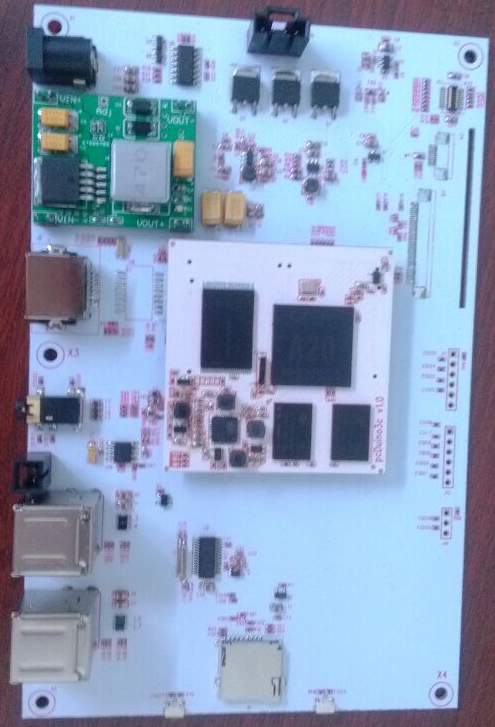
\includegraphics[keepaspectratio=true,angle=0,height=1.0\textheight,width=1.0\textwidth]{corebaseboard-foto-1.png}
\caption{Core (center) and Base Board Photo}
\label{fig:bbfoto}
\end{figure}


\section{Specifications}
Specs, Core Board:

\begin{itemize}
  \item{Allwinner A20 ARM Processor}
  \item{1GHz CPU}
  \item{1 Gig RAM}
\end{itemize}

Specs, Base Board:
\begin{itemize}
  \item{MicroSD Card Slot}
  \item{4 USB A Ports}
  \item{Line level audio in/out}
  \item{Amplified audio out (mono speaker headers)}
  \item{Ethernet}
  \item{MIPI/CSI Camera socket}
  \item{10 GPIO pins}
  \item{24V power input}
  \item{12V RGB LED Strip driver}
  \item{uBoot button}
  \item{RST button}
  \item{DBG UART Pins}
  \item{LVDS LCD Socket}
  \item{I2C Touch screen socket}
\end{itemize}

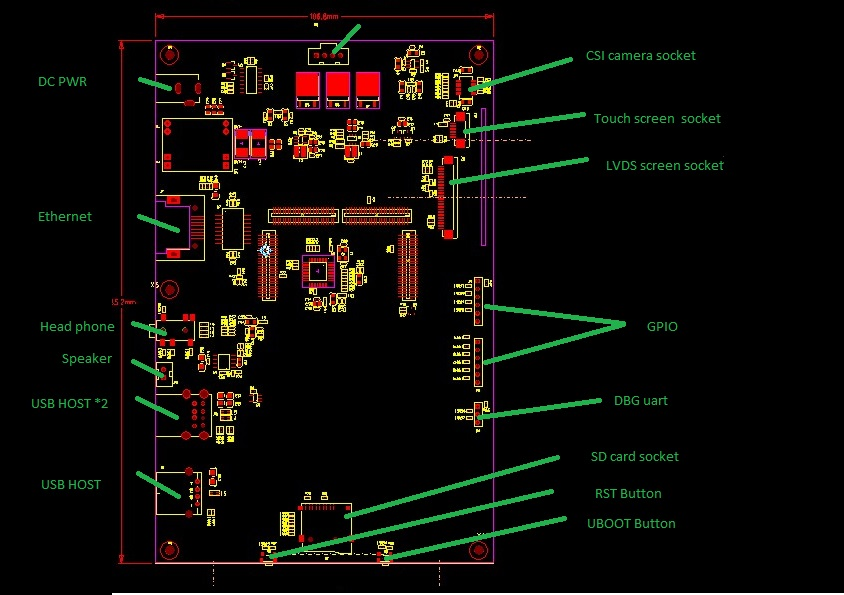
\includepdf[addtolist={1,figure,{Base Board Layout},bblay},pages=-,landscape=true,reflect=false,turn=true,fitpaper=true,keepaspectratio=true]{baseboard_layout_linksprite_20140630.jpg}

\section{Other Hardware}

\subsection{LCD}
The LCD screen will mount near the EZGNU. The board is being specified by
Linksprite.

Specs LCD:

\begin{itemize}
  \item{1280x800 Resolution}
  \item{LVDS interface}
\end{itemize}


\subsection{LED Lights}
There will be RBG LED strips to indicate various printer states via colored
lights.

\subsection{Camera}
The first version won't have a camera, though the EZGNU does have a header for
common types.

